\section{ANÁLISE DE MARCHA}


\subsection{BREVE HISTÓRICO} 

Conforme \citeonline{Baker2007}, Aristóteles (384-322 A.C.) pode ser considerado o primeiro a registrar comentários a respeito de como os humanos caminham. 
O autor ainda afirma que só na renascença houve progressos através de experimentos e teorizações, feitas principalmente por Giovanni Borelli (1608-1679). Jules Etienne Marey (1830-1904), trabalhando na França e Eadweard Muybridge (1830-1904), trabalhando na América, fizeram grandes avanços na área de mensuração.
Ainda conforme \citeonline{Baker2007}, os maiores avanços no início do século vinte foram os desenvolvimentos das placas de força e o entendimento da cinética da marcha.

Na obra de \citeonline{Muybridge1885}, de antes do século vinte, ele busca sistematizar maneiras de se analisar o movimento humano, principalmente usando técnicas de fotografia. 
A obra apesar de ser o resultado das pesquisas do autor, tem um valor artístico inegável.  
A Figura \ref{inicio_corrida} dá o tom da obra.

\begin{figure}[ht]
	\centering
	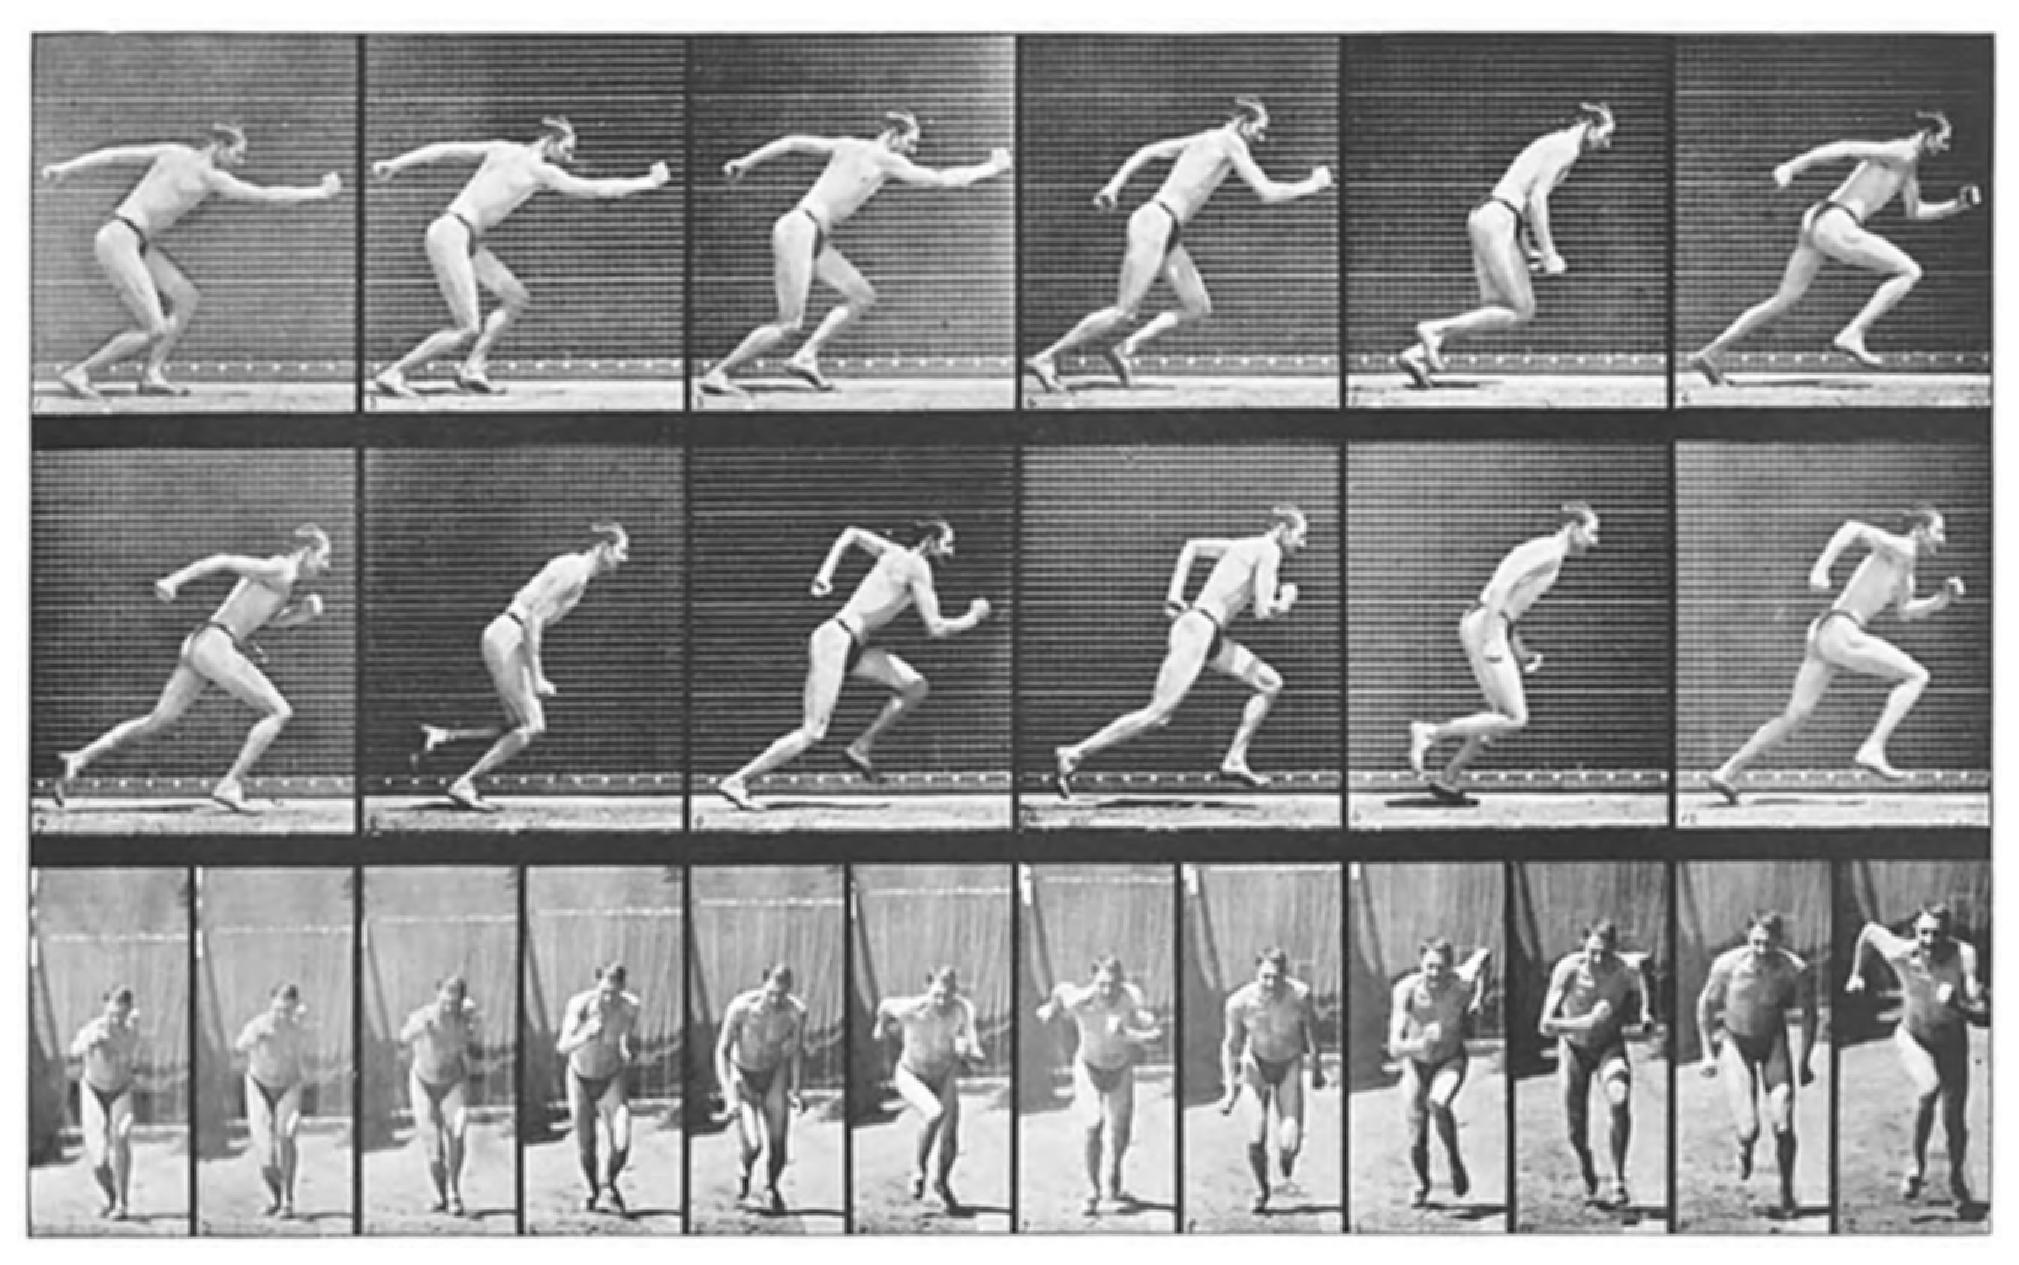
\includegraphics[width=15cm]{figuras/inicio_corrida.eps}
	\caption{Atleta iniciando uma corrida. Fonte: \citeonline{Muybridge1885}.}
	\label{inicio_corrida}
\end{figure}


Apesar dos avanços ocorridos na análise de marcha até meados do meio do século vinte, foi só após o advento dos computadores modernos que a análise de marcha clínica tornou-se amplamente disponível \cite{Baker2007}.



\subsection{FUNDAMENTOS}
Segundo \citeonline{Perry2010}, para se classificar as diferentes divisões da marcha é necessário separá-las em períodos, fases e tarefas, conforme a Figura \ref{fases_marcha}.

\begin{figure}[ht]
	\centering
	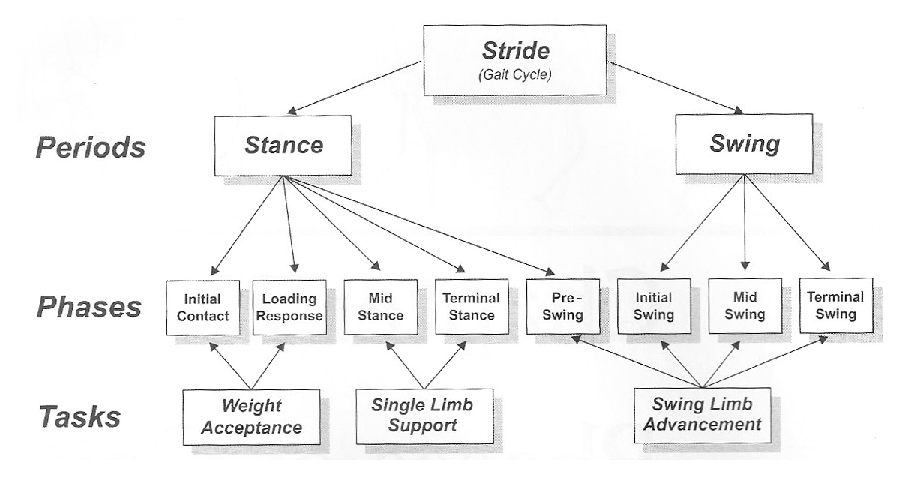
\includegraphics[width=15cm]{figuras/fases_marcha.eps}
	\caption{Divisões do Ciclo de Marcha. Fonte: \citeonline{Perry2010}.}
	\label{fases_marcha}
\end{figure}

A passada, que também é um sinônimo para um ciclo de marcha completo, equivale ao momento que, por exemplo, o pé direito toca o chão, sai do chão e o toca novamente. Dentro do ciclo de marcha temos também os períodos que são dois, apoio e balanço. 
O apoio corresponde ao período que o pé toca o chão pela primeira vez e o deixa durante o ciclo. 
O balanço é o período que o mesmo pé deixa o chão e o toca novamente iniciando um novo apoio \cite{Perry2010}. 

Além dos períodos, como vemos na Figura \ref{fases_marcha}, temos as fases. As fases representa um intervalo, percentual durante o ciclo da marcha e são muito importantes na avaliação do ciclo, 
pois grandes variações nos sinais durante alguma fase, pode representar algum distúrbio a ser diagnosticado. São oito as fases \cite{Perry2010}:
\begin{enumerate}
	\item Contato inicial, corresponde de 0 a 2\% do ciclo de marcha;
	\item Resposta à carga, corresponde de 2\% até 12\% do ciclo de marcha;
	\item Apoio médio, corresponde de 12\% até 31\% do ciclo de marcha;
	\item Apoio terminal, corresponde de 31\% até 50\% do ciclo de marcha;
	\item Pré-balanço, corresponde de 50\% ate 62\% do ciclo de marcha;
	\item Balanço inicial corresponde de 62\% até 75\% do ciclo de marcha;
	\item Balanço médio corresponde de 75\% até 87\% do ciclo de marcha;
	\item Balanço terminal corresponde de 87\% até 100\% do ciclo de marcha. 
\end{enumerate}

As tarefas são as funções desempenhadas durante o ciclo de marcha e estão relacionadas especificamente com as fases. 
A Figura \ref{fases_marcha} mostra o relacionamento entre as três tarefas e suas fases específicas. São elas \cite{Perry2010}:
\begin{enumerate}
	\item \emph{Aceitação de Peso} - Ela é responsável pela absorção do choque, estabilidade inicial de membro e preservação da progressão;
	\item \emph{Apoio Simples} - Esta tarefa é responsável por manter um membro apoiado no chão e progredindo o ciclo de marcha, até que o outro membro toque o chão, ou seja, sua função, é fazer que um membro suporte todo o peso do corpo sozinho;
	\item \emph{Avanço do Membro} - Sua função é avançar o membro que está no período de balanço, até que ele esteja pronto para fazer um novo contato inicial.
\end{enumerate}

\subsection{MÉTODOS DE COLETA DE DADOS PARA ANÁLISE} 
\label{metodos_analise}

Esta seção descreve alguns dos dispositivos que podem ser usados para coletar dados de movimentos. 
Estes podem ser convertidos e usados pelo software desenvolvido, desde que uma adaptação seja feita. 
No momento de conclusão deste trabalho o único método adaptado é o por captura de dados por câmeras, usando o sistema da \emph{Qualisys}.

\textbf{Captura de dados por câmeras}

\noindent
Pode-se começar este assunto pelos métodos de mensuração de movimentos espaciais e de ângulos.
O método mais sofisticado hoje para análise de movimentos é o baseado em câmaras de vídeo. 
Inclusive \citeonline{Grip2013}, demonstra discorre sobre as vantagens dos sistemas de câmeras ópticas usando marcadores de superfície em detrimento de outras técnicas de captura de movimento. 
Neste tipo de técnica, os marcadores podem ser ativos ou passivos, a diferença é que os ativos emitem algum tipo de sinal luminoso ou infravermelho, por exemplo. 
Este método permite visualizar a posição espacial dos marcadores e a partir daí, calcular velocidades, acelerações, ângulos, velocidades angulares, acelerações angulares, etc.
A Figura \ref{oqus_mri} mostra o modelo \emph{Oqus MRI} da \emph{Qualisys}. Esta é uma câmera muito utilizada no mercado não só para análise clínica mas também para captura de movimentos para serem inseridos em filmes e jogos de computador. 
Já a Figura \ref{visao_qtm} mostra o software QTM do mesmo fabricante, já com os dados capturados e animados na tela do computador.
A Figura \ref{markers} é uma visão de uma possível configuração de câmeras, capturando marcadores de superfície passivos de um paciente.

\begin{figure}[H]
	\centering
	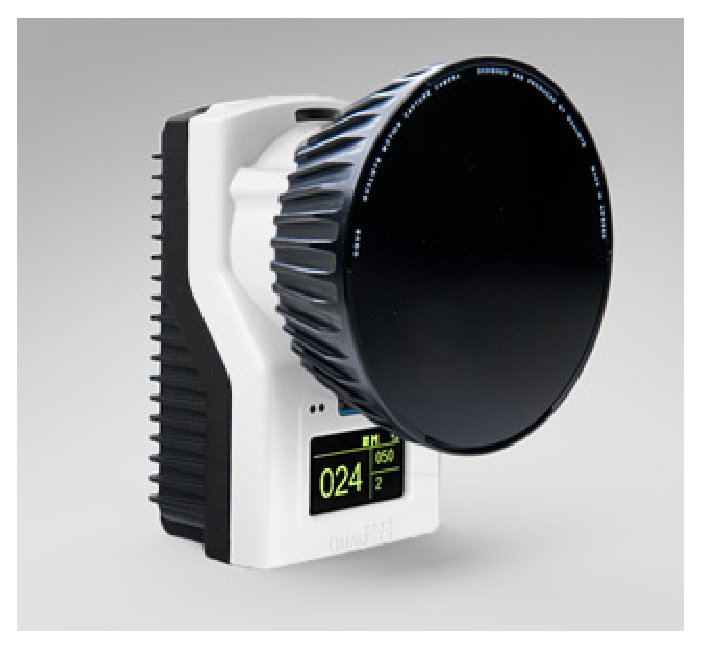
\includegraphics[width=7cm]{figuras/oqus-mri.eps}
	\caption{Câmera Oqus MRI. Fonte: \citeonline{Qualisys2013}.
}
	\label{oqus_mri}
\end{figure}


\begin{figure}[H]
	\centering
	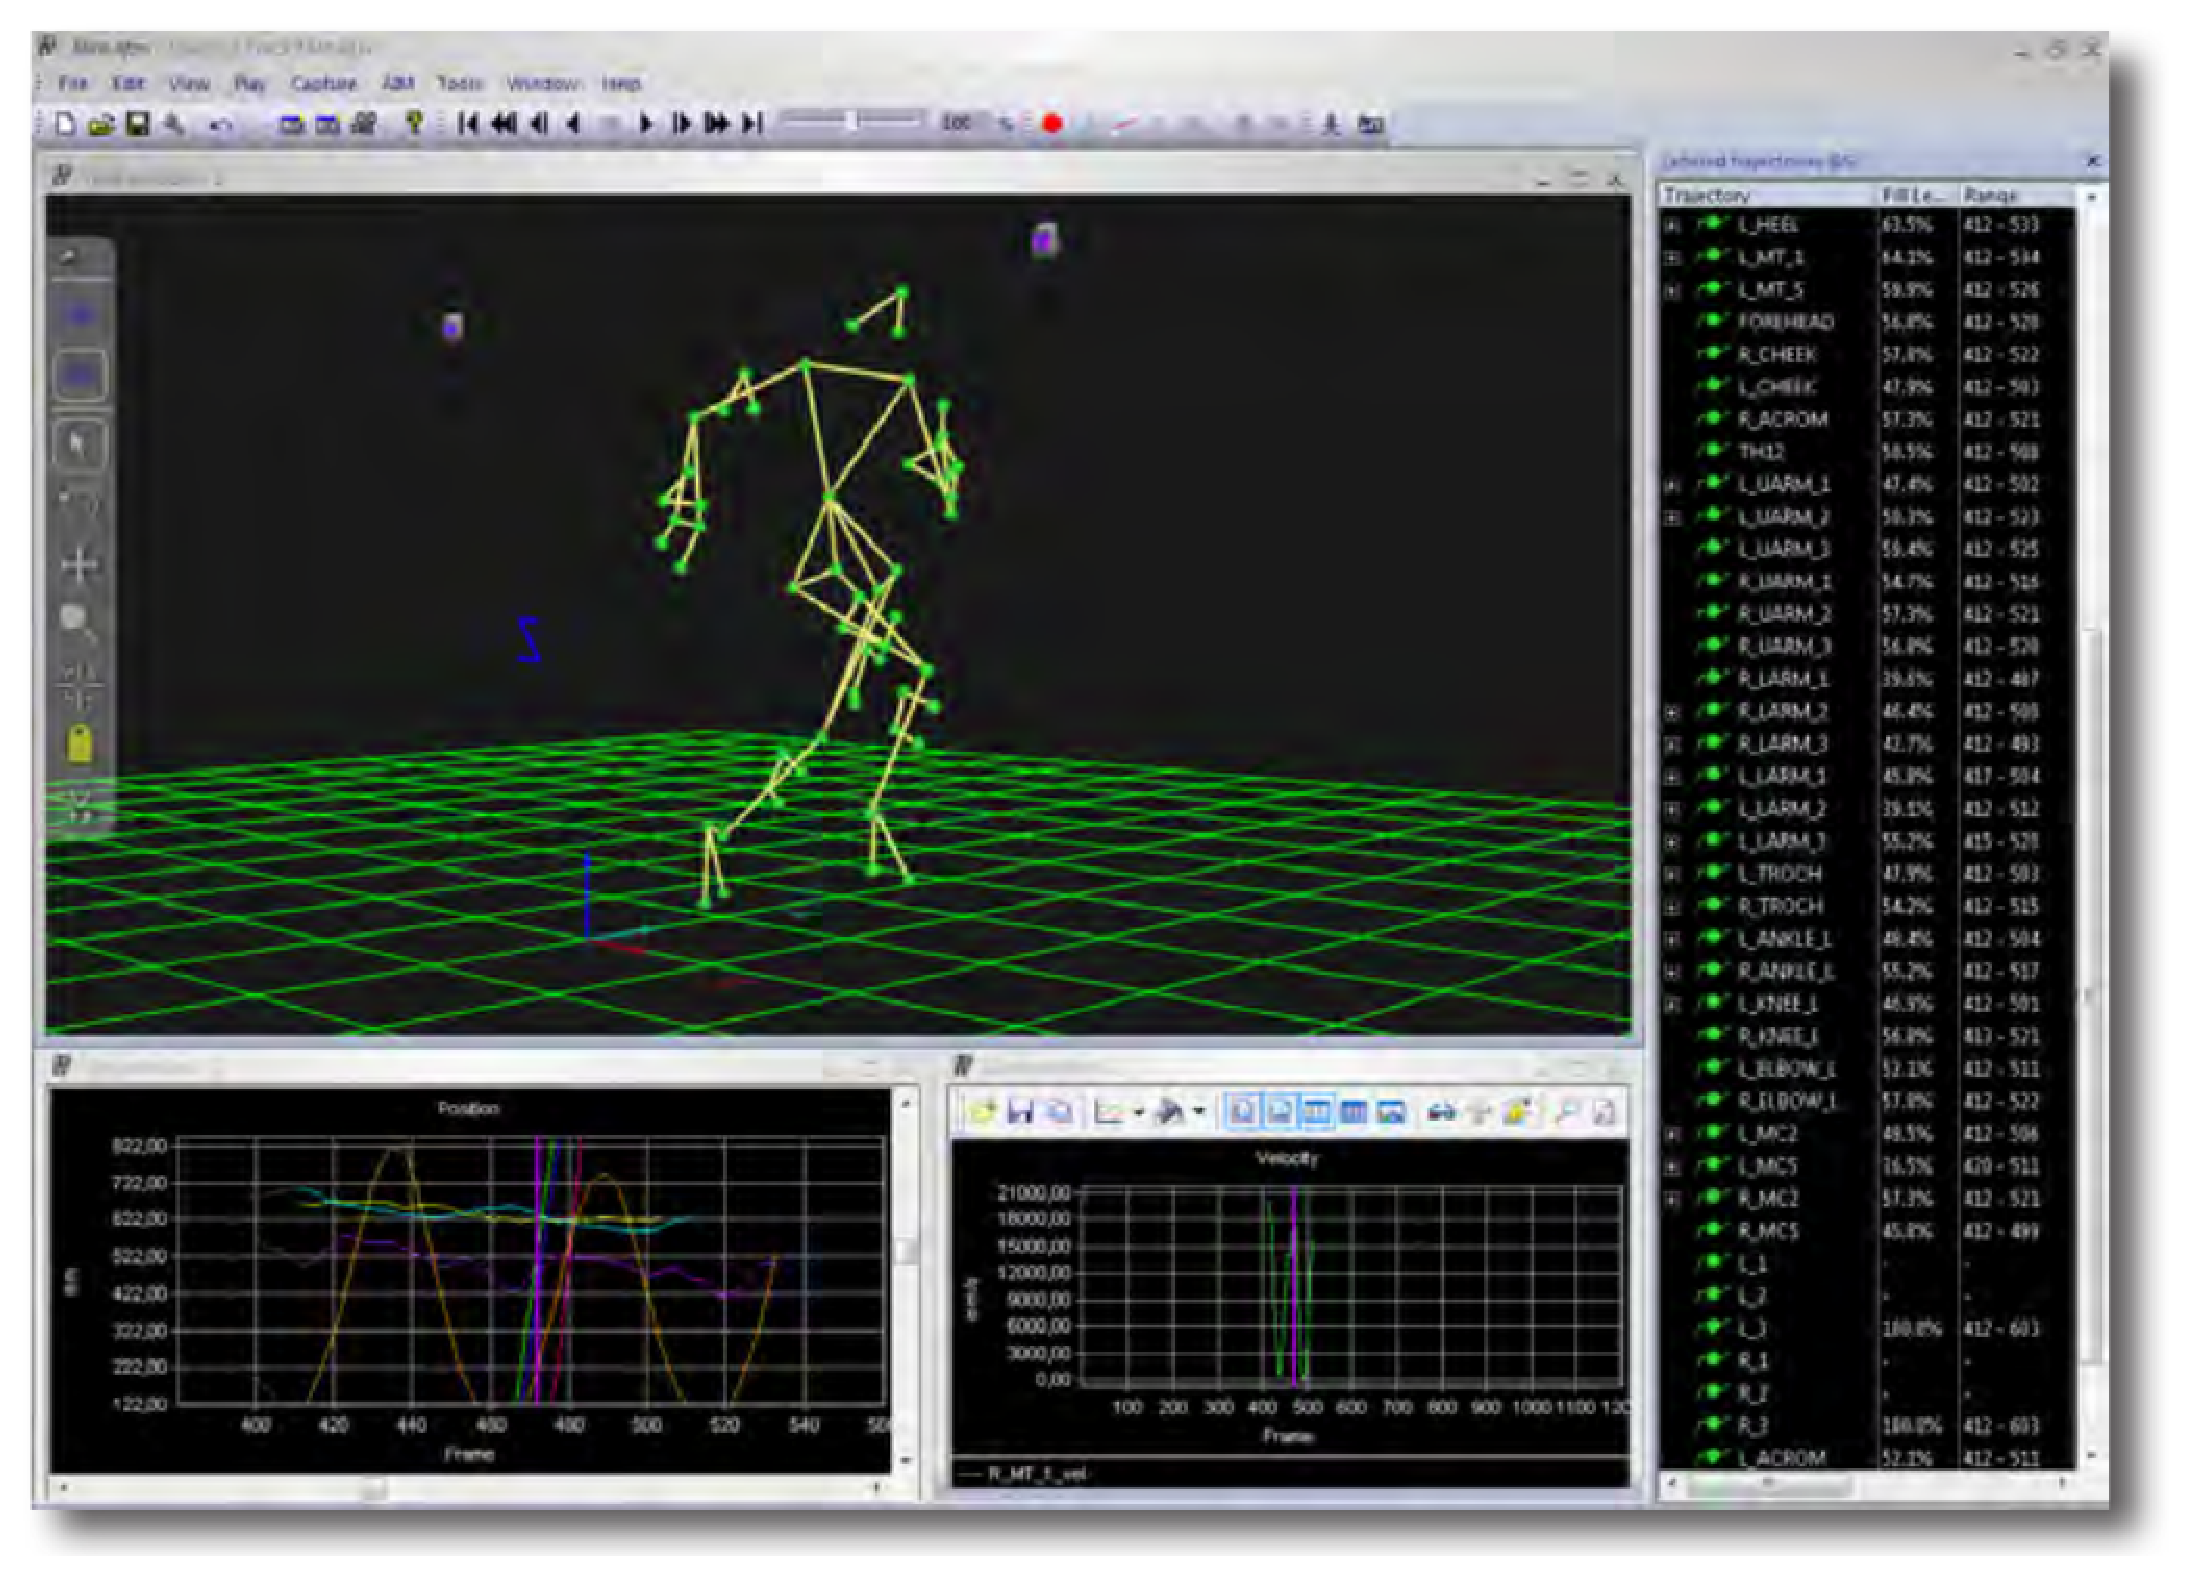
\includegraphics[width=15cm]{figuras/qtm.eps}
	\caption{Visão do QTM. Fonte: \citeonline{Qualisys2010}.}
	\label{visao_qtm}
	
\end{figure}


\begin{figure}[H]
	\centering
	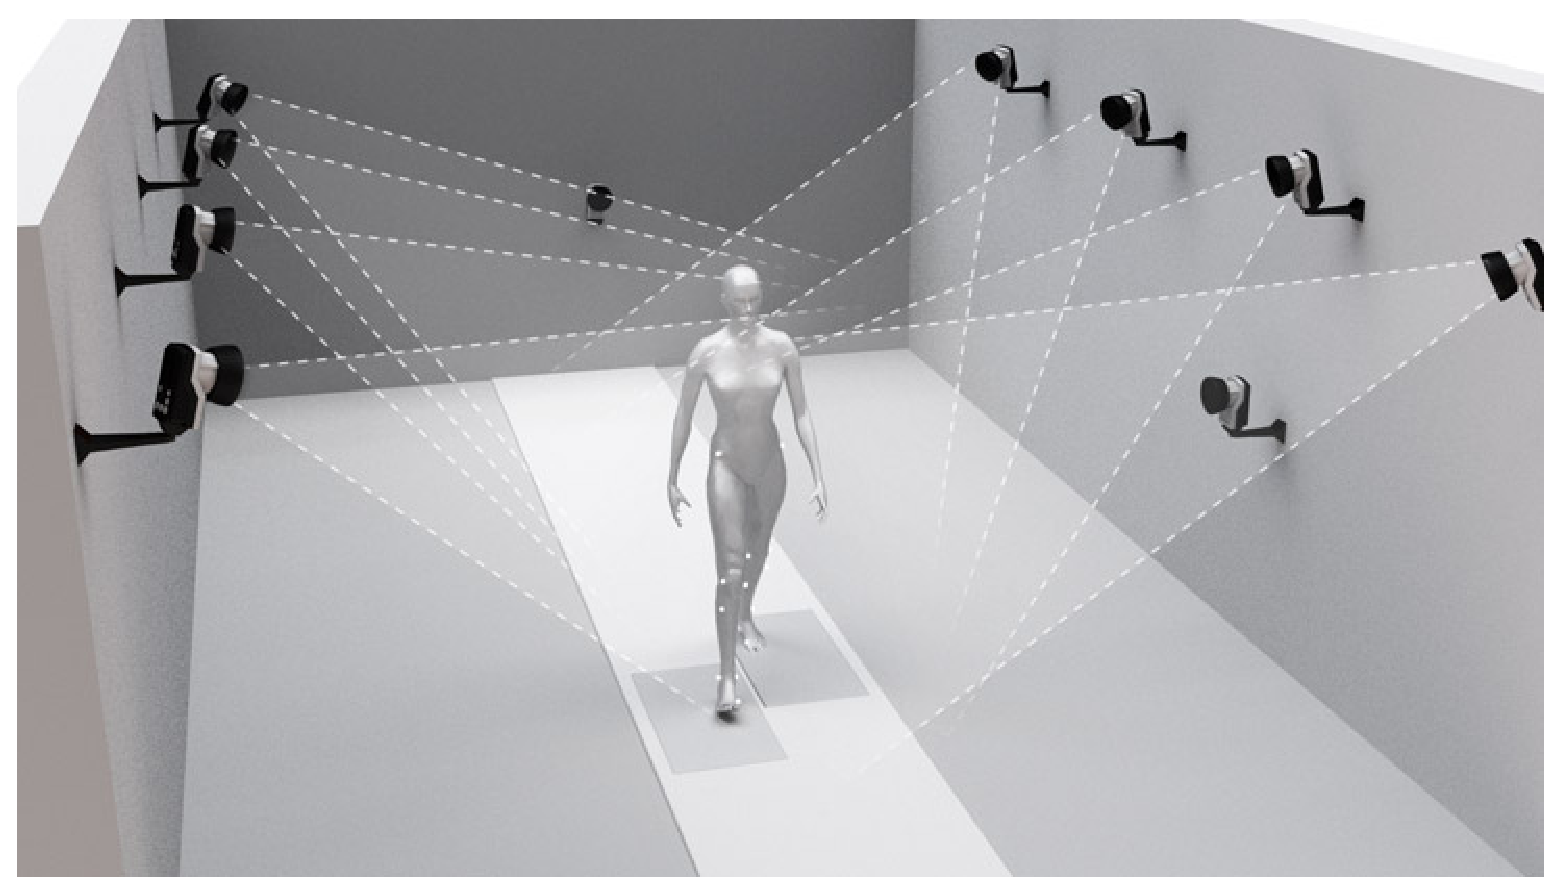
\includegraphics[width=14cm]{figuras/markers.eps}
	\caption{Configuração de câmeras para captura de dados de marcadores passivos fixados no paciente. Fonte: \citeonline{Qualisys2013a}.}
	\label{markers}
	
\end{figure}


\textbf{Captura por Unidade de Medida Inercial}

\noindent
Uma outra alternativa, que está sendo desenvolvida na FGA/UnB, é um dispositivo baseado em uma Unidade de Medida Inercial \emph{(Inertial Measurement Unit - IMU)}. O IMU é um dispositivo eletrônico provido de acelerômetrose um magnetômetro.
Segundo \citeonline{Leite2014}, esta é uma alternativa não visual para extrair parâmetros cinemáticos da marcha humana, trajetória e velocidade. 
O trabalho foi realizado comparando-se os resultados fornecidos pelo dispositivo e captura de vídeo.
A Figura \ref{imu} mostra um experimento onde o vídeo e os dados do \emph{IMU} são coletados ao mesmo tempo.


Na Figura \ref{imu2}, é possível visualizar o resultado dos dados coletados do \emph{IMU} e da câmera. 
Veja que é um resultado bem promissor. 
Mas a maior vantagem do dispositivo, ainda não foi discutida, seu baixíssimo valor em relação a solução com várias câmeras.

\begin{figure}[H]
	\centering
	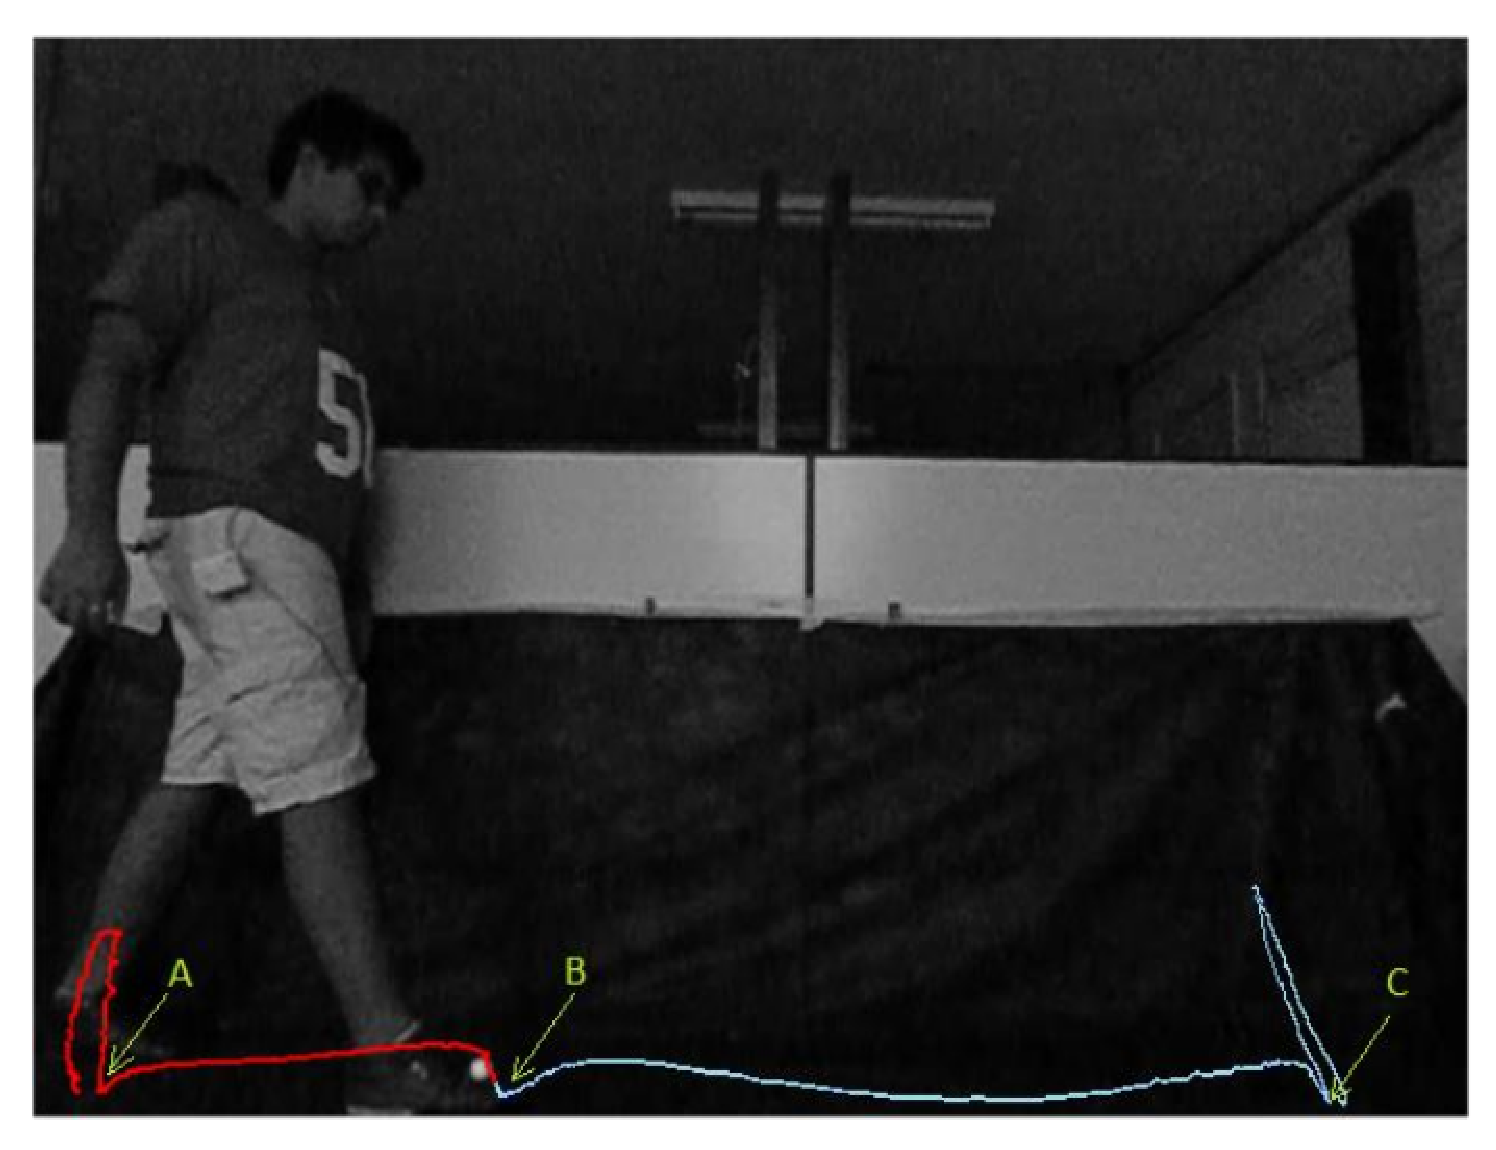
\includegraphics[width=7cm]{figuras/imu.eps}
	\caption{Experimento de captura de dados de \emph{IMU} em conjunto com uma câmera. Fonte: \citeonline{Leite2014}.}
	\label{imu}
	
\end{figure}


\begin{figure}[H]
	\centering
	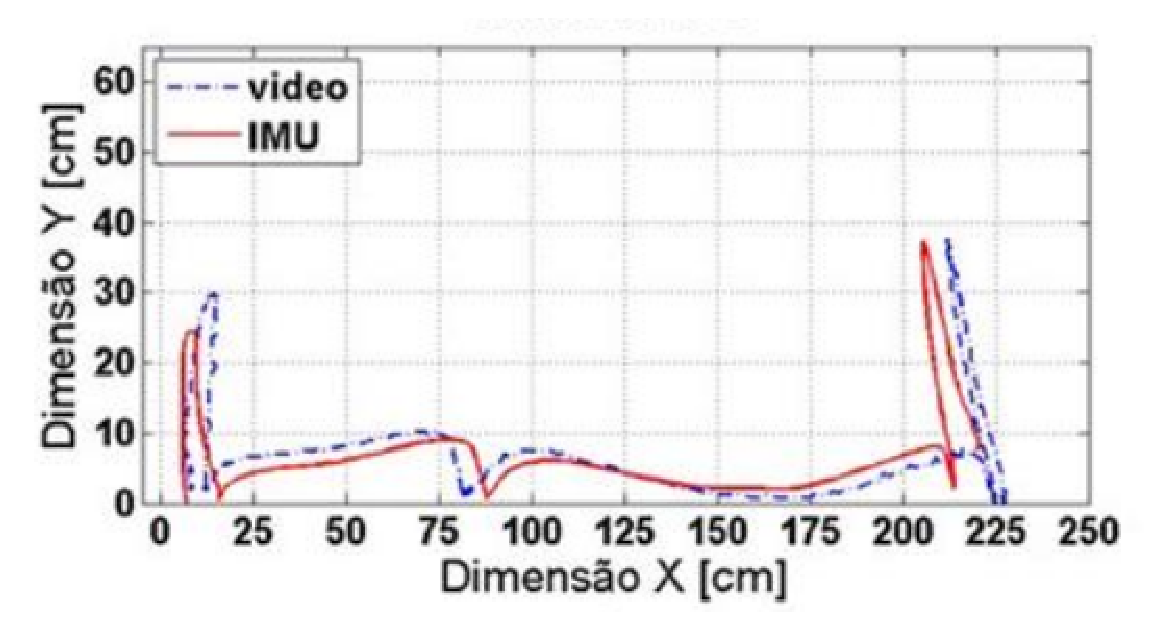
\includegraphics[width=10cm]{figuras/imu2.eps}
	\caption{Comparação entre \emph{IMU} e a câmera. Fonte: \citeonline{Leite2014}.}
	\label{imu2}
	
\end{figure}



\textbf{Captura por Eletrogoniômetros}

\noindent
Eletrogoniômetros são também usados para capturar angulações em articulações, basicamente este aparelho provê uma voltagem que é representativa da mudança de ângulo entre duas superfícies, nas quais o dispositivo é fixado \cite{K.Ibrahim2012}. 
A principal vantagem deste dispositivo é que seu custo é baixo. A Figura \ref{egn} mostra um exemplo de eletrogoniômetro.
Ele tem como desevantagem sua pouca precisão, mas ainda assim pode ser usado na análise de movimentos por software.



\begin{figure}[H]
	\centering
	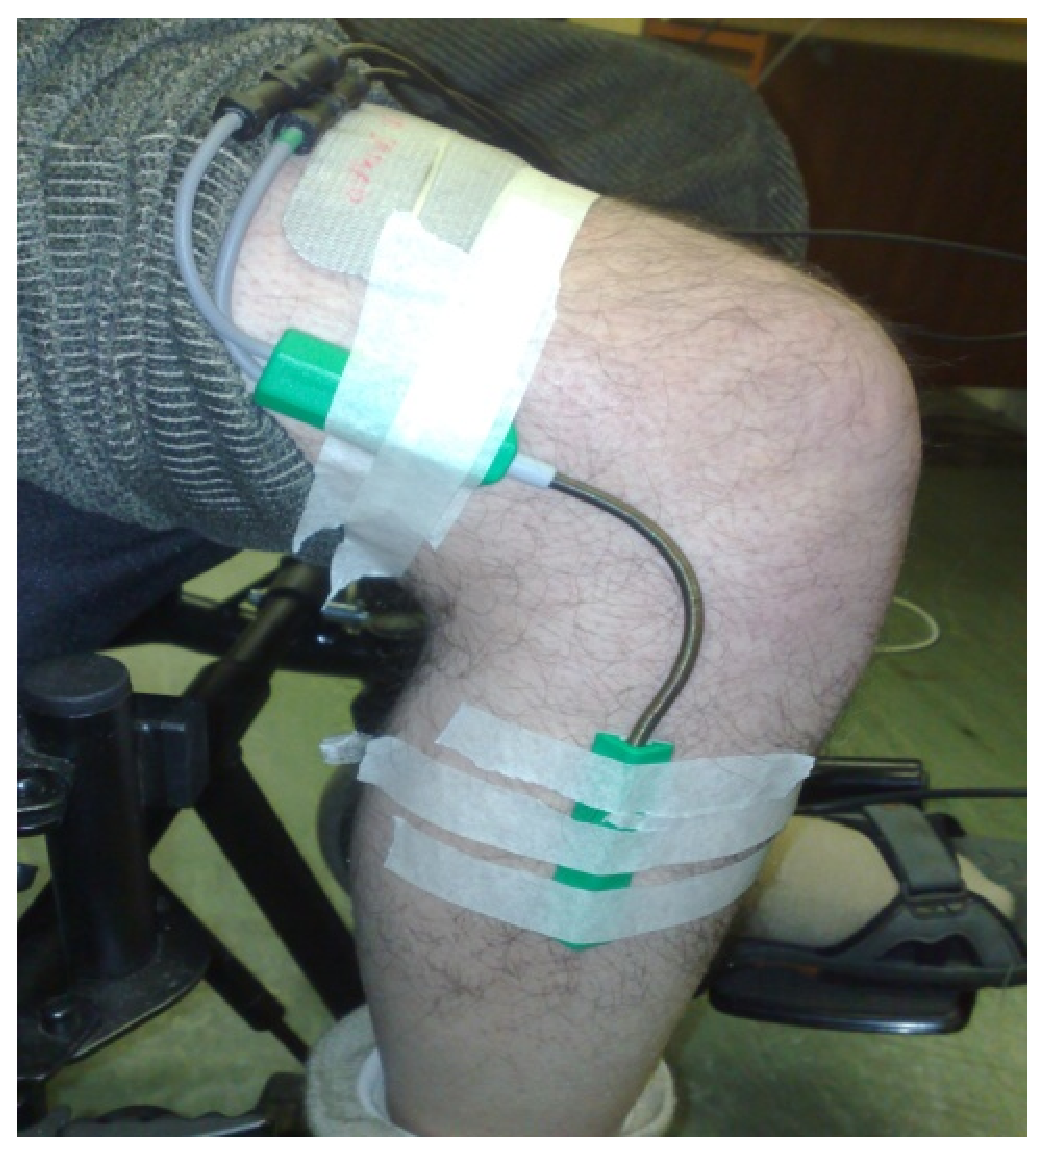
\includegraphics[width=7cm]{figuras/egn.eps}
	\caption{Eletrogoniômetro. Fonte: \citeonline{K.Ibrahim2012}.}
	\label{egn}
	
\end{figure}


